%\vspace{-0.1in}
\section{Challenges}
\label{sec:challenges}

\subsection{Working with existing routing protocols}
\label{sec:incremental}

Most of the current proposals~\cite{tcpbolt, karol2003prevention,
sancho2004,lash,wu2003fault} for deadlock avoidance are based on custom routing
protocols that go to great lengths to avoid CBD.  Unfortunately, this makes it
very difficult, if not impossible to deploy them in existing data center
networks. 

Modern data centers are built atop Ethernet and IP. Routing is accomplished in a
variety of ways, including BGP~\cite{vl2, facebookrouting} or using SDN-like
protocols~\cite{singh2015jupiter}.  No matter what routing protocols are used,
data center operators tune them carefully satisfy numerous requirements such as
manageability and fault tolerance.  In addition, operators invest heavily in
tools and technologies to monitor and maintain their networks.

Thus, it is very difficult for a data center operator to substantially change their routing
infrastructure in order to avoid deadlocks. This task appears especially
onerous because RoCEv2 itself can be deployed without any changes to routing
protocols -- RoCEv2 packets are encapsulated in normal UDP packets are routed
like any normal IP packets.

Thus, unlike prior work, \sysname{} requires no changes to the underlying routing
protocol.

\subsection{Data Center Networks are Dynamic}\label{sec:reroute}

Building a deadlock avoidance scheme that does not make any changes to routing
protocols is easier said than done. The key problem is that the routing is
dynamic -- paths can change in response to link failures or load.

\begin{figure}
	%\vspace{-0.1in}
	\centering
	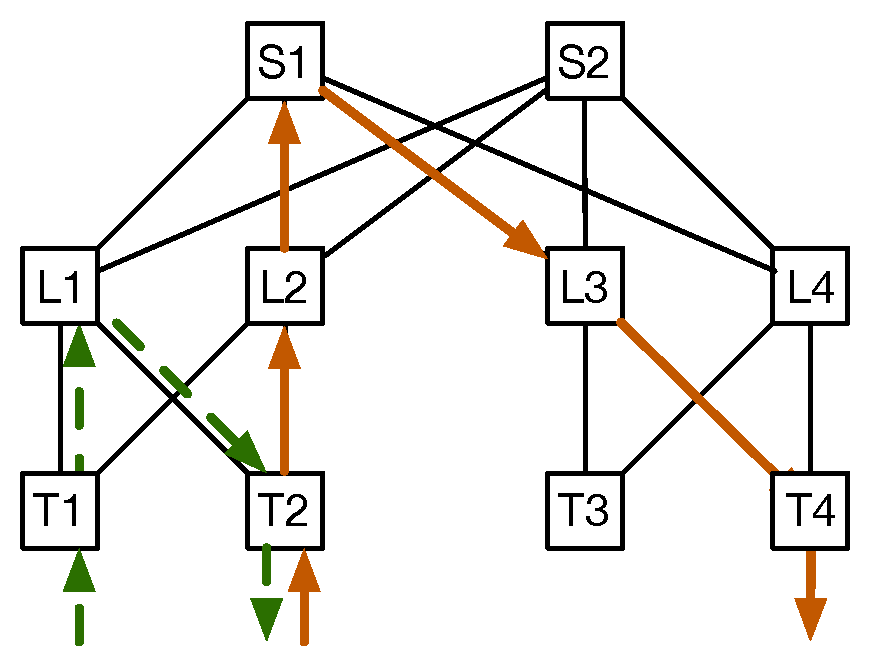
\includegraphics[width=0.4\textwidth] {figs/up-down}
	\caption{UP-DOWN routing in a Clos network.}\label{fig:up-down}
\end{figure}

Take {Figure~\ref{fig:up-down} as an example. It shows a simplified (and small) version of
network deployed in our data center. If packets always follow so-called
up-down (also called valley-free~\cite{qiu2007toward}) routing, then deadlock
cannot happen as CBD is not possible. In up-down routing, a packet first goes UP
from the source server to one of the common ancestor switches of the source and
destination servers, then it goes DOWN from the common ancestor to the
destination server.  In UP-DOWN routing, the following property holds: when the
packet is on its way UP, it should not go DOWN; when it is on its way DOWN, it
should not go UP.

%\begin{figure}
	%\vspace{-0.1in}
	%\centering
	%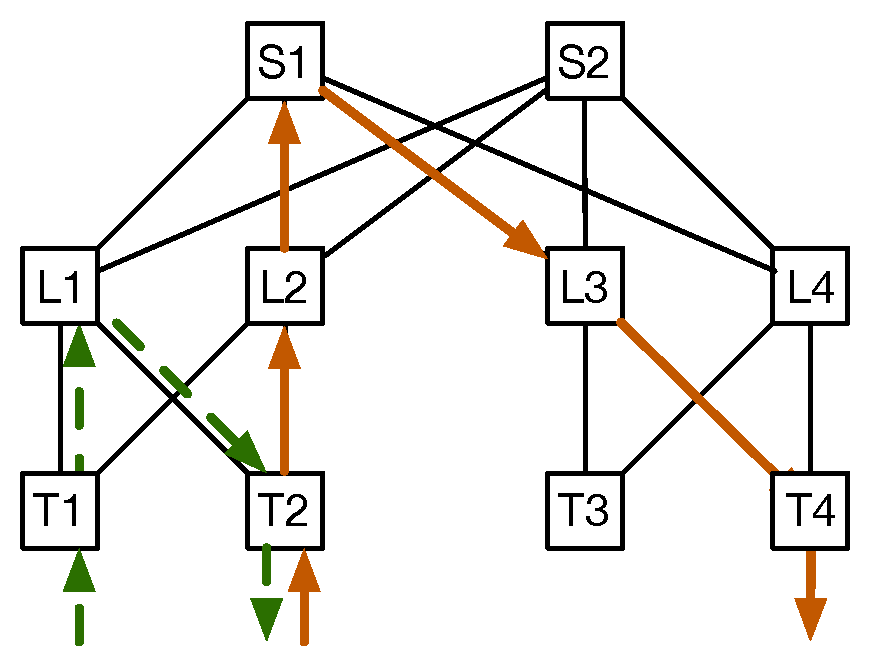
\includegraphics[width=0.4\textwidth] {figs/up-down}
	%\caption{Violation of up-down routing can lead to deadlocks}
	%\label{fig:up-down-deadlock}
%\end{figure}

However, packets may deviate from the UP-DOWN paths due to several reasons
including software errors on routers, link flapping, routing protocol
flapping~\cite{f10}. As have shown in~\cite{shpiner2016unlocking}, when the
UP-DOWN property is broken and packets may reroute multiple times between two
layers of switches, and deadlocks may form as a result, as shown in
Figure~\ref{fig:priority_transition}(a).

We regularly observe deviations from up-down routing in our data centers.  We
see hundreds of such routes per day, and they can persist for minutes or even
longer. Overall, we estimate that $0.001\%$ of the traffic is routed over such
paths. This may sound tiny, but given that our network carries petabytes of
traffic per day, the absolute amount of traffic affected by such routing is
quite high. This makes the threat of deadlocks, as discussed
in\cite{rdmaatscale,shpiner2016unlocking,hu2016deadlocks} quite real.

%% In this paper, we show our measurement results from a large cloud computing
%% provider that UP-DOWN routing property does break in reality and packets can be
%% rerouted with a non negligible probability.
%% 
%% Our measurement works as follows. We instrument the servers to send out IP-in-IP
%% packets to the high-layer switches. The outer source and destination IP
%% addresses are set to the sending server and one of the high layer switches, and
%% the inner source and destination IP addresses are set to the switch and the
%% sending server, respectively. The high-layer switches are configured to
%% decapsulate those IP-in-IP packets that are targeting themselves in hardware.
%% 
%% After decapsulation, the outer IP header is discarded, and the packet is then
%% routed using its inner header. We set a TTL value, 64 in this paper, in the
%% inner IP header. As the packet is forwarded back to the server, the TTL is
%% decremented per hop. For a three-layer Clos network, there are three hops from
%% the highest layer switches to the server. Hence normally the TTL value of the
%% received packets should be 61.
%% 
%% If, however, the TTL value of a received packet is smaller than 61, say 59, we
%% know the received packet was not taking the shortest path, and the packet must
%% have taken a reroute path.
%% 
%% In this paper, for every measurement, a server sends out $n=100$ IP-in-IP
%% probing packets, if the received TTL values are not equal, we know packet
%% reroute happened for this measurement. We then calculate the reroute probability
%% of the measurements as $\frac{M}{N}$, where $M$ is the number of measurements
%% that experienced packet reroute, and $N$ is the total number of measurements. We
%% carried out the measurements for one week in more than 20 data centers. The
%% measurement results are shown in Table~\ref{fig:reroute}.
%% 
%% \begin{table}[t]
%% \begin{small}
%% \begin{center}
%% \begin{tabular}{|r|r|r|c|}
%% \hline    Date    & Total No.  & Rerouted No.   & Reroute probability \\
%% \hline 11/01/2016 & 11381533570 & 148416 &  1.3e-5 \\
%% \hline 11/02/2016 & 11056408780 & 130815 &  1.2e-5 \\
%% \hline 11/03/2016 & 10316034165 & 104472 &  1.0e-5 \\
%% \hline 11/04/2016 & 10273000622 & 92555  &  0.9e-5 \\
%% \hline 11/05/2016 & 10230003382 & 102872 &  1.0e-5 \\
%% \hline 11/06/2016 & 10491233987 & 106266 &  1.0e-5 \\
%% \hline 11/07/2016 & 9608289622  & 100916 &  1.1e-5 \\
%% \hline
%% \end{tabular}
%% \end{center}
%% \caption{Packet reroute measurements in the data centers of a large cloud computing service provider.}\label{fig:reroute}
%% \end{small}
%% \end{table}
%% 
%% The most important conclusion we can draw from Table~\ref{fig:reroute} is that
%% packet reroute does happen in data center networks. The reroute probability is
%% around $10^{-5}$. Though $10^{-5}$ is not a big number, given the large traffic
%% volume and the large scale data center networks, the deadlocks due to packet
%% reroute as discussed in \cite{rdmaatscale,shpiner2016unlocking,hu2016deadlocks}
%% do not just exist in paper designs. They are real!
%% 
%% Therefore how to address potential deadlocks due to packet reroute becomes a pressing challenge.

%adding discussions on why packet reroute happen.

\subsection{Limited Number of Lossless Queues}
\label{subsec:pfcheadroom}

One easy way to avoid deadlock without changing routing is to buffer packets
from each flow separately from other flows at each hop -- essentialy putting
each flow in its own class, and applying per-hop backpressure only within the
class.  A more sophesticated scheme in~\cite{karol2003prevention} requires as
many priorities as the diameter of the network. 

One obvious problem with this idea is that the PFC standrad supports only 8
priority classes. But a bigger problem is that a switch can support only a small
number of lossless queues.

The number of lossless queues that a switch can support is limited by two
factors. First, the commodity switching ASICs typically support only a small
number of queues (e.g., eight) and we need to use some of the queues for the
lossy traffic. Second, to guarantee the lossless property, a switch needs to
reserve certain amount of {\it headroom} from the memory pool. The size of the
memory pool is of limited size, hence the number of lossless queues is further
limited by the size of the memory pool.

The reserved headroom per port per lossless queue is to absorb the packets in
flight from the time a receiver decides to send a PFC pause frame to its
upstream sender to the time the sender stops transmitting after receiving the
pause frame. See \cite{rdmaatscale} for how PFC works. We describe how the
headroom size is calculated in Appendix \ref{APPHEADROOM}.

From Appendix \ref{APPHEADROOM}, we can see that for a typical 32-port 40GbE
Ethernet switch, it needs to reserve 2.76MB memory as the headroom to support
one lossless queue. For a switch of 12MB memory, this is 23\% of the total
memory.

The headroom calculated in Appendix \ref{APPHEADROOM} is to make sure that
packets cannot be dropped. In practice, the reservation size should be larger
than that. This is because we need some additional reservation to make sure that
the link is not under-utilized, when the receiver releases the sender from been
paused. Furthermore, we need to reserve buffers for lossy traffic, which is
still the dominating traffic in data centers. Consider all these constrains, the
number of lossless queues can be supported by the current commodity switches
typically is limited to two.

We note that new switching ASICs may be able to support more lossless queues by
adding more memory, using smaller cell size (64-byte), reducing the pause frame
response time. But the widely deployed switches support only two lossless
queues. It is unlikely that the switches can support more than four or five
lossless queues. Hence the solutions that use a large number of lossless queues
are not practical. 

We now describe how \sysname{} addresses these three challenges. 
